\documentclass[letterpaper]{report}
\usepackage{fullpage}
\usepackage{graphicx}
%\usepackage{color}
\usepackage{courier}
\usepackage[usenames,dvipsnames,svgnames,table]{xcolor}
\usepackage{amsmath}
\usepackage{amssymb}
\usepackage{url}
\usepackage{listings}
\usepackage{hyperref}
\usepackage{hypcap}
\usepackage{makeidx}
\hyphenation{Semant-Eco}
\lstdefinestyle{Java}{
language=Java,
breaklines=true,
basicstyle=\scriptsize\ttfamily,
keywordstyle=\bfseries\color{violet},
commentstyle=\itshape\color{green!60!black},
stringstyle=\color{blue}
}
\lstdefinestyle{XML}{
language=XML,
breaklines=true,
basicstyle=\scriptsize\ttfamily
}
\makeindex
\begin{document}
\title{SemantEco: A Modular Framework for Integration of Ecological, Environmental, and Earth Sciences Data}
\author{Evan W. Patton \\
Tetherless World Constellation\\
Rensselaer Polytechnic Institute\\
110 8th Street\\
Troy, NY 12180, USA\\
\texttt{pattoe@rpi.edu}
\and Patrice Seyed \\
University of New Mexico\\
1 University Boulevard\\
Albuquerque, NM 87131, USA\\
\texttt{seyeda2@rpi.edu}
\and Deborah L. McGuinness\\
Tetherless World Constellation\\
Rensselaer Polytechnic Institute\\
110 8th Street\\
Troy, NY 12180, USA\\
\texttt{dlm@cs.rpi.edu}
}
\maketitle
\begin{abstract}
In this paper we discuss the architecture of SemantEco, a modular framework for integrating data from ecological, environmental, and Earth sciences. The architecture of SemantEco encapsulates features as modules that can be combined to present data in different ways. We provide an in-depth discussion on module implementation as well as detail the existing modules available in SemantEco and how they interact with one another. The architecture is generalizable to other domains as well. % crap, I know
\end{abstract}

\renewcommand{\abstractname}{Acknowledgements}
\begin{abstract}
The Tetherless World Constellation is supported in part by Fujitsu, Lockheed Martin, LGS, Microsoft Research, Qualcomm, in addition to sponsored research from DARPA, IARPA, NASA, NSF, and USGS. Evan W. Patton is supported by an NSF Graduate Research Fellowship.
\end{abstract}

\renewcommand{\abstractname}{Licensing}
\begin{abstract}
SemantEco is made available under the {\color{red} Apache License v2.0}. This documentation is made available under the terms of {\color{red} Creative Commons BY-SA 3.0 Unported License}.
\end{abstract}

\tableofcontents

\cleardoublepage
\listoffigures
\addcontentsline{toc}{chapter}{\listfigurename}

\cleardoublepage
\listoftables
\addcontentsline{toc}{chapter}{\listtablename}

\cleardoublepage
\lstlistoflistings
\addcontentsline{toc}{chapter}{\lstlistlistingname}

\chapter{Introduction}
\label{introduction}
% The following is taken verbatim from the introduction to the FGCS paper. It should be adapted as necessary to fit a tech report.
In many places around the world, wildlife and the habitats on which they depend are deteriorating. For instance, almost 40 percent of the United States' freshwater fish species are considered at risk or vulnerable to extinction according to~\cite{fish}. Aiming at preserving the environment and wildlife, scientists and resource managers have initiated various efforts to monitor ecological and environmental trends, investigate causes and possible effects of pollution, and identify threats to wildlife and their habitats. To be effective, these efforts must be undertaken with a large scale and multidisciplinary perspective.  However, by nature this approach requires access and use of disparate data sources and systems. For example, the USGS provides integrated science and technology to support resource managers in the U.S. Department of the Interior (DOI) through initiatives such as the Wyoming Landscape Conservation Initiative (WLCI): an effort to assess and enhance aquatic and terrestrial habitats at a landscape scale in southwest Wyoming. Decision support systems are one end result of scientific research that facilitates examination of the many tradeoffs and conflicting drivers that resource managers often wade through in their work, from energy and agricultural development to fish and wildlife conservation to recreational uses of public lands. 

Meanwhile, semantic science and technologies have been used in environmental monitoring to facilitate knowledge encoding, data integration and collaborative scientific workflows~\cite{environmental-modelling}. Previously we proposed the Tetherless World Constellation Semantic Ecology and Environment Portal (SemantEco) \cite{SemantAqua:ISWC2011,SemantAqua:Wang-MSThesis} as both an environmental portal application and as an example of a semantic infrastructure for environmental informatics applications. The portal captures the semantics of domain knowledge using a family of ontologies, integrates environmental data (e.g. water quality measurement and regulatory data), infers pollution events using OWL2 inference, and leverages provenance. In this paper, we extend the focus of SemantEco beyond water quality and related human health effects to a more comprehensive effort that includes fish and wildlife species and their related health effects. As such, this extension is in concert with the “One Health” concept, defined as ``the collaborative effort of multiple disciplines — working locally, nationally, and globally — to attain optimal health for people, animals and the environment'' \cite{one-health}. Consider a data manager interested in identifying correlations between declines of a bird population observed in a river due to chemicals released by nearby factories. There may be direct causal links (i.e. pollutant X in a diet kills Y) or indirect links (e.g. pollutant X causes reproductive system changes leading to lowered breeding success and resultant population declines). To identify these scenarios, resource managers need access to a number and variety of information and data sources including databases containing species observation counts, literature on the environmental effects of pollutants, how species may migrate and interact with one another, and so forth. Semantic technologies will facilitate access to multidisciplinary information that will aid resource managers in making decisions about complex ecosystems. These technologies also enhance reusability and address extensibility issues targeting challenges in the areas of data integration, provenance, and scalability.

We use semantic technologies to provide responses to these challenges. This work presents a new architecture\index{architecture!SemantEco} that evolves an existing water quality portal into a general model for performing ecological and environmental data integration across many different data sources and domains. Additionally, this new architecture is designed to be horizontally scalable through the use of representational state transfer \cite{REST}. We also demonstrate how semantic technologies can be used to encourage interoperability by connecting one existing well-used observation schema - the Extensible Observation Ontology (OBOE) \index{ontology!Extensible Observation}\index{OBOE|see{ontology, Extensible Observation}}\cite{OBOE} to support interoperable observation data. We investigated the reasoning implications of adopting OBOE for interpreting data and found out that OBOE brings greater interoperability at the cost of longer reasoning time. Additionally, we now integrate various ecological and environmental data: wildlife observational data from the Avian Knowledge Network (AKN\footnote{http://www.avianknowledge.net/}) and U.S. Geological Survey (USGS\footnote{http://www.usgs.gov/}); environmental criteria for wildlife from the Environmental Protection Agency (EPA\footnote{http://www.epa.gov/}); water body data from USGS; and health effects of contaminants on wildlife from Wildpro\footnote{http://wildpro.twycrosszoo.org/}. These are provided in addition to the existing water quality and regulatory data presented in earlier versions of this work. Our approach provides a formal encoding of the semantics of the data and provides services for automatic reasoning and visualizations. Furthermore, we compared the performance of a standard semantic web reasoner used in previous iterations with a new, customized rule based reasoner over our data. Lastly, we enhanced the provenance support of the existing portal by incorporating rationale as provenance. This extensibility enabled by semantic technologies allows the portal to consume data from many different domains and present it together for the purposes of informing environmental stakeholders.

\section{Definitions}
SemantEco is an amalgamation of many different ontologies and as such this technical report includes a number of detailed items. This section provides a number of definitions for common terms that readers will encounter throughout this document.

\begin{itemize}
\item SemantEco Framework - the conceptualization of SemantEco as a modular framework that combines different modules into a single application
\item SemantEco servlet\index{servlet!SemantEco} - a Java Servlet 3.0 Specification-compatible servlet that implements the SemantEco Framework
\item SemantEco module\index{module!SemantEco} - a JAR file containing a compiled implementation of the Module interface and supporting resources such as JavaScript (JS), Cascading Stylesheets (CSS), and Java Servlet Pages (JSP) or HTML content
\item jQuery - An extensible JavaScript library that provides powerful features for web application developers
\item AJAX - Asynchronous Javascript and XML, a process by which web applications make calls to a server to obtain data while the user can continue to interact with the current web page
\item BBQ - jQuery Back button and Query library; useful for providing navigation and state features in single-page web applications
\item RDF - The Resource Description Framework defined by the World Wide Web Consortium
\item OWL - The Web Ontology Language, in this work we make use of OWL 2 DL
\item Model - A programmatic construct provided by the Jena Semantic Web framework to access and manipulate an RDF graph
\item POM - Project Object Model, an XML language for representing a project, its dependencies, and how it is built and tested
\item Artifact - The product of a maven compilation, usually a Java Archive (JAR) file containing compiled code and any resources
\item Repository - A collection of artifacts and metadata provided by a POM file
\item Maven module\index{module!Maven} - An collection of code that will generate a Maven artifact and can be grouped with related projects based on directory structure
\end{itemize}

\section{Where To Begin}
Readers interested in getting a general overview of how SemantEco is structured architectural should be able to read this document in order. Chapters are arranged such that having an understanding of earlier chapters provides a general background for future chapters. For readers interested in the application flow from a server perspective, Section \ref{servlet} introduces the SemantEco servlet\index{servlet!SemantEco} and how it is initialized server side. For readers interested in the client-side application flow, Section \index{User Interface!index.jsp}\ref{index.jsp} introduces the SemantEco interface described in its index.jsp and walks through how it and the other user interface components operate.

\chapter{Architecture Design}
\label{architecture}\index{architecture!SemantEco|textbf}
In this chapter we will discuss the architecture of the new SemantEco, from its adherence to the Java Servlet Specification\index{servlet!specification} so that it can be deployed in many different environments to its method of executing modules and queries to accomplish user tasks. We will also discuss how the RESTful\index{Representational State Transfer}\index{REST|see{Representational State Transfer}} client-server communication works to enable SemantEco both as a web application and as a web service.

\section{The SemantEco Servlet}
\label{servlet}
SemantEco is, at its core, a Java Servlet 3.0\footnote{http://jcp.org/aboutJava/communityprocess/final/jsr315/index.html} servlet\index{servlet!SemantEco|textbf}. As such, it can be deployed into a number of servlet containers\index{servlet!containers|textbf}, such as Tomcat,\footnote{http://tomcat.apache.org/} Jetty,\footnote{http://jetty.codehaus.org/jetty/} and Glassfish.\footnote{http://glassfish.java.net/} In this way, system administrators can easily deploy SemantEco alongside existing servlet-based services and reduce overall system maintenance. Previous versions of SemantEco used a built-in HTTP server and were thus less flexible for deployment as it would need to be proxied\index{proxy} through a forward-facing web server such as Apache.\footnote{http://httpd.apache.org/}. While proxying is no longer necessary, it can still be beneficial for deployments where speed is important as a proxy can cache SemantEco's responses.

The SemantEco servlet is, at its core, a `plug-and-play' architecture. The servlet mostly provides glue code that is responsible for combining functionality of different modules. A \textit{module} is a self-contained Java Archive that provides functionality to SemantEco via different methods. The specifics of how modules work will be discussed in Chapter~\ref{writing-modules}.

\subsection{Initialization of SemantEco on Deployment} 
When the servlet container starts or when a developer uses the maven tomcat7:deploy goal, the first action taken after the SemantEcoServlet is constructed is a call by the container to the init method per the Java Servlet 3.0 specification. During this initialization, SemantEco configures any missing directories, initializes its logging system (log4j), and sets up the module manager, which includes loading all prepackaged modules in the Web archive (war) file.

\subsection{Special URL Patterns}
\label{url-patterns}
The SemantEco responds to a number of URL patterns\index{URL!patterns|textbf} that require custom processing. These include:
\begin{itemize}
\item \texttt{/js/config.js} -- Client configuration specific to the SemantEco deployment, including the base URL for the deployment and where to submit RESTful calls.
\item \texttt{/js/modules/*} -- Autogenerated JavaScript files to facilitate client-server communication (see Section~\ref{client-server-comm}).
\item \texttt{/log} -- WebSockets interface for sending debugging data to client.\footnote{As of this writing there is no standardization for WebSockets in Java Servlet 3.0 so this functionality is limited to Tomcat 7+ servers that support HTTP Protocol upgrades via Apache Coyote.}
\item \texttt{/rest/*} -- RESTful calls to SemantEco modules (see Section~\ref{client-server-comm}).
\end{itemize}

\noindent If a request is made to the servlet, these special URLs are handled in the servlet's \texttt{doGet} method. Otherwise, the servlet container will attempt to retrieve the file named by the URL. If no such file exists than an HTTP 404 error will be generated.

\section{The Module Manager}
\label{module-manager}\index{ModuleManager@\texttt{ModuleManager}|textbf}\index{ModuleManager@\texttt{ModuleManager}|(}
SemantEco modules are maintained by a class called the \texttt{ModuleManager}. The \texttt{ModuleManager} is responsible for loading modules from their JAR files and configuring them. If a module is removed from SemantEco, the \texttt{ModuleManager} will delete the module instance and unload the module files from the class path. The \texttt{ModuleManager} is also responsible for constructing the user interface and semantic models and modifying queries before they are executed. It accomplishes these tasks by consulting the available modules.

\subsection{Installing Modules}
\label{installing-modules}\index{module!SemantEco!installing}
\texttt{ModuleManager} uses the Apache Virtual File System\footnote{http://commons.apache.org/vfs/} to actively monitor the modules directory and respond to the addition or deletion of modules. During servlet initialization, the \texttt{ModuleManager} will actively scan the directory and fire addition events for each module available at that time to bootstrap the entire process. When a module is added the following steps occur:

\begin{enumerate}
\item The \texttt{ModuleManager} instantiates a \texttt{ModuleClassLoader} object responsible for reading in the JAR file and defining the classes in the JAR with the Java Virtual Machine. It also performs validation that at least one of the classes in the JAR represents a implementation of the \texttt{Module} interface.
\item The \texttt{ModuleManager} `explodes' the JAR by extracting everything in the META-INF/res/ directory into the web application's resources directory under a module-specific directory to prevent naming clashes between modules. This directory is named the same as the JAR without the `.jar' extension.
\item The \texttt{ModuleManager} instantiates an instance of each \texttt{Module} implementation found in the jar.
\item The \texttt{ModuleManager} installs the newly created \texttt{Module} to its internal store.
\item The \texttt{ModuleManager} instantiates a \texttt{ModuleConfiguration} for each new module and loads the modules.properties file into the configuration for the module if one exists. This configuration is then supplied to the module via its \texttt{setModuleConfiguration} method.
\end{enumerate}

If during the initialization process an error occurs while processing the JAR's classes the module will not be instantiated and the \texttt{ModuleClassLoader} will be destroyed. If the module throws an exception in its constructor, then it will not be added to the list of available modules, \textbf{\textit{but its code will not be unloaded}}.

\subsection{Uninstalling Modules}
\label{uninstalling-modules}\index{module!SemantEco!uninstalling}
If a module is not needed or is acting faulty it can be removed from the system. When the module's JAR file is removed from the modules directory, the Apache Virtual File System will send the \texttt{ModuleManager} a message that the file has been removed, in which case the following steps occur:

\begin{enumerate}
\item 
\end{enumerate}

\subsection{Visiting Modules}
The Module Manager encapsulates access to the various modules available to SemantEco and employs the visitor pattern to interact with the modules. The specifics of how to implement a module's visit methods are discussed in more detail in Section~\ref{visitors}. For the various core components, such as the \texttt{Request} object or the \texttt{QueryExecutor}, the Module Manager exposes a number of public methods:

\begin{itemize}
\item buildUserInterface(SemantEcoUI, Request)\index{User Interface!build method} - When an instance of the \texttt{SemantEcoUI} object is instantiated (usually in response to having to render one of the tag library components, see Section~\ref{tag-library}), it is passed to the \texttt{ModuleManager} using this function, which in turn calls each visit(SemantEcoUI, Request) method on all of loaded modules.
\item buildOntologyModel(OntModel, Request)\index{Ontology Model!build method} - When the \texttt{QueryExecutor} requires the ontology model prior to executing a reasoning query, it generates an \texttt{OntModel} via Jena's \texttt{ModelFactory} and passes it along with the active \texttt{Request} object to this method. The \texttt{ModuleManager} then calls the visit methods of all of the \textit{active modules}\footnote{An active module is a module that does not declare a domain or has at least one domain enabled in the Domain facet}.
\item buildDataModel(Model, Request)\index{Data Model!build method} - When the \texttt{QueryExecutor} requires a data model prior to executing a reasoning query, it generates a Model and proceeds in a similar manner as buildOntologyModel defined above. This method only calls a module's visit method if it is an active module.
\item augmentQuery(Query, Request, Module)\index{query!augmenting} - When the QueryExecutor\index{QueryExecutor@\texttt{QueryExecutor}} intends to execute a query, either remotely or locally, it calls this method and passes the Query, the current Request object, and the calling Module. This method will visit each active module via its visit(Query, Request) method, assuming that module is not the same as the calling module to prevent loops where a module's visit method may spawn further queries.
\end{itemize}
\index{ModuleManager@\texttt{ModuleManager}|)}

\section{ModuleConfiguration}
\index{ModuleConfiguration@\texttt{ModuleConfiguration}|textbf}
When each module is instantiated by the \texttt{ModuleManager}, the \texttt{ModuleManager} passes the module an instance of \texttt{ModuleConfiguration} via the module's \texttt{setModuleConfiguration} method. Modules that wish to execute queries or retrieve runtime information about available domains, etc., should save the reference to the \texttt{ModuleConfiguration} object.

The \texttt{ModuleConfiguration} object provides a number of useful methods for the module:

\begin{itemize}
\item\textbf{getSparqlEndpoint} - Retrieves the default SPARQL endpoint that will execute queries for this module. This can be overridden by calling a \texttt{QueryFactory}'s \texttt{execute} method that takes an endpoint URL.
\item\textbf{getQueryFactory} - Obtains a \texttt{QueryFactory} the module can use to instantiate \texttt{Query} objects.
\item\textbf{getQueryExecutor} - Obtains a \texttt{QueryExecutor} the module can use for executing queries either on remote endpoints (such as the default endpoint returned by getSparqlEndpoint) or the local model after all modules have populated it with content relevant to the actively processed \texttt{Request} object. The \texttt{QueryExecutor} object is discussed in more detail in Section~\ref{query-executor}.
\item\textbf{getResource} - Obtains a reference to a resource in the module's \texttt{META-INF/res} directory so that it can be added to the user interface.
\item\textbf{generateStringResource} - Generates a resource object from a string; this is primarily used for generating dynamic content based on SPARQL queries.
\item\textbf{getLogger} - Gets the default Apache log4j\footnote{http://logging.apache.org/log4j/1.2/} Logger for the module.
\item\textbf{getDomain} - Gets or creates a \texttt{Domain} object for a given URI; this should only be called by modules that also implement \texttt{ProvidesDomain} (note: SemantEco does not enforce this but interaction with domains are limited if a module is not also an implementation of \texttt{ProvidesDomain}).
\item\textbf{listDomains} - Returns a \texttt{java.util.List} of all domains know to SemantEco at the time it is called.
\end{itemize}

\section{The Query Executor}
\label{query-executor}\index{QueryExecutor@\texttt{QueryExecutor}|textbf}
The \texttt{QueryExecutor} interface provides the primary method for modules to query the SemantEco knowledge base and interact with external SPARQL services via the Query object. It also provides methods for properly forming HTTP requests to external services to ease in module development by hiding many of the details related to calling remote services. Each QueryExecutor implementation must implement the following public methods:

\begin{itemize}
\item execute(Query) - Executes the specified query against the default endpoint and returns the response as a String.
\item execute(Query, Model) - Executes the specified query against the default endpoint and loads the response into the provided Jena model. This method only is valid for Query objects that are of type CONSTRUCT or DESCRIBE and thus return an RDF graph.
\item execute(String, Query) - Executes the specified query against the specified endpoint and returns the response as a String.
\item execute(String, Query, Model) - Executes the specified query against the specified endpoint and loads the response into the provided Jena model. The conditions on execute(Query, Model) also apply here.
\item getDefaultSparqlEndpoint() - Returns the default SPARQL endpoint. This will either be the SemantEco default or the module specific endpoint specified in the module's properties file (see subsection~\ref{installing-modules}).
\item accept(String) - Adds a MIME type to the Accept HTTP header, e.g. "application/json" or "text/turtle". This returns a clone of the QueryExecutor with appropriate modifications so that calls can be chained together to add multiple types and immediately perform an execution.
\item executeLocalQuery(Query) - Performs a local query over the knowledge base by obtaining the combined model via the current Request object (see subsection~\ref{request-object}).
\end{itemize}

For most modules, the general flow of information involving the \texttt{QueryExecutor} proceeds in the following way:

\begin{enumerate}
\item Construct a \texttt{Query} object and add appropriate triple patterns.
\item If the query is a CONSTRUCT or DESCRIBE query, construct a Jena \texttt{Model} object via Jena's \texttt{ModelFactory}.
\item Set the appropriate accept header using \texttt{accept()} and then call the appropriate execute method, e.g. \texttt{config.getQueryExecutor().accept("application/json").execute(myQuery);}
\end{enumerate}

Prior to execution of a query, the \texttt{QueryExecutor} calls the \texttt{ModuleManager}'s \texttt{augmentQuery(Query, Request, Module)} method. This causes the \texttt{ModuleManager} to pass each \texttt{Module} the query object so that they may add any additional triple patterns based on the parameters passed in the current state (encapsulated within the \texttt{Request} object). Modules are visited in the order that they were instantiated by the \texttt{ModuleManager} when the servlet was initialized. The final \texttt{Module} parameter is used by the \texttt{ModuleManager} to ensure termination by preventing an infinite loop in the event a \texttt{Module} creates and executes a \texttt{Query} from within its own \texttt{visit(Query, Request)} method---it is assumed that a \texttt{Module} has done everything it needs to do to construct the query prior to executing it.

\section{Client-Server Communication}
\label{client-server-comm}
In this section we will discuss how SemantEco uses the \texttt{@QueryMethod} annotation in order to generate communication code between client and server. 

\subsection{Query Methods}
To facilitate interaction between SemantEco clients and the SemantEco server, the framework provides an annotation for module designers called \texttt{QueryMethod} that allows the designer to identify Java methods that should be callable from client-side code. For each module with at least one \texttt{QueryMethod}, the framework will provide a \texttt{<script>} element in index.jsp under the \texttt{/js/modules/} path mentioned in Section~\ref{url-patterns}. The browser will attempt to load this script from this URL, which prompts SemantEco to generate the necessary glue code to support the call. This operation is done in the JavaScript generator.

\subsubsection{The JavaScript Generator}
The JavaScript generator is a utility class that is responsible for standardizing the client-server communication code to limit potential errors on the part of module designers. Each module has its \texttt{QueryMethod}s exposed in exactly the same way and any requests to these methods from the clients are processed in exactly the same way by the SemantEco servlet. The general flow of the JavaScript generator is as follows:

\begin{enumerate}
\item Begin by generating an empty JavaScript object assigned to a variable with the same name as the Java class.
\item For a given module, use the Java Reflect API to obtain a list of all methods defined on the module.
\item For each method, examine its annotation set to determine if the method has the \texttt{QueryMethod} annotation.
\item If the method is annotated as a \texttt{QueryMethod}, add a key/value pair to the JavaScript object in \#1 where the key is the name of the method and the value is a function that takes a dictionary of arguments, a success function, and an optional error function and performs the following actions:
\begin{enumerate}
\item Extend the SemantEco state with any optional arguments given in the arguments parameter. If an argument appears in both the state and the arguments object, the value in the arguments is used.
\item Using jQuery, execute an Asynchronous JavaScript and XML (AJAX) to the server at a predetermined URL in the form of \texttt{/rest/<module-name>/<method-name>}.
\item Set the success and error handlers on the AJAX request so the appropriate functions are called when the request completes.
\end{enumerate}
\item If at least one method was a \texttt{QueryMethod} return the final object back to the servlet so it can be sent to the client, otherwise return nothing.
\end{enumerate}

\subsubsection{The Request Object}
\label{request-object}
When a \texttt{QueryMethod} is called from a client, it is intercepted by the SemantEco servlet's \texttt{doGet} method. This method identifies the request as a RESTful call to a module and proceeds to parse the parameters sent by the client into the appropriate types. This information is then encapsulated in a \texttt{Request} object (realized by the \texttt{ClientRequest} class) that can be passed to the module/method combination identified in the URL. In addition to providing modules access to the parameters of a REST call, the \texttt{Request} object also provides the following methods:

\begin{itemize}
\item\textbf{getLogger} - Gets an Apache log4j Logger customized for the specific request if the client sent a valid identifier for a known WebSocket outbound channel (see Section~\ref{debugging-techniques} for more details).
\item\textbf{getModel} - Gets the \texttt{OntModel} containing all of the ontologies for every active module based on the \textbf{Request}'s parameters. If the \texttt{OntModel} has not yet been constructed, this will cause one to be created and the \texttt{ModuleManager} will call each active module's \texttt{visit(OntModel)} method.
\item\textbf{getDataModel} - Gets the \texttt{Model} containing all of the data for every active module based on the \textbf{Request}'s parameters. If the \texttt{Model} has not yet been constructed, this will cause one to be created and the \texttt{ModuleManager} will call each active module's \texttt{visit(Model)} method.
\item\textbf{getCombinedModel} - Gets a combined \texttt{Model} that contains the contents of both the ontology model and data model. If either model has yet to be built this will construct the missing models first following the steps above.
\end{itemize}

It is important to note that the results of each of the above methods caches its results until the processing of the \texttt{Request} completes, i.e. multiple calls to these methods will not incur any additional time penalties after the model is first built.

\section{Debugging Techniques}
\label{debugging-techniques}
This section discusses some of the debugging techniques that designers can use in the construction and debugging of modules.

\subsection{Web Sockets}
To ease debugging server behavior during client actions, SemantEco uses the Web Socket specification to open up a persistent connection between the client and server if the client supports it. This occurs during the client's initialization procedure. If the Web Socket initialization is successful, the SemantEco servlet stores a reference to the socket and sends back a hash of the socket's reference that the client stores in a cookie. In future requests, the servlet will attempt to read the cookie and, if the hash identifies an open socket, will use that socket to generate a \texttt{LoggerWrapper} object that wraps the \texttt{Request}'s default logger and sends copies of all log statements to the client. Log statements received on the client via the Web Socket are printed to the client's console. Messages may still be blocked if the log level on the server is too high for the type of log required (e.g. the developer wishes to see DEBUG messages but the server is configured for INFO and higher).

\subsection{Remote Java Debugging}
In addition to using a Logger object to log events as they occur, it is also useful for designers to step through code and examine variables to identify potential logic issues and correct them. Because SemantEco uses the Maven build system it is generally the case that Eclipse does not recognize it as a servlet. Therefore, debugging the servlet is a more involved process than general servlet development done entirely in Eclipse. To debug SemantEco one should do the following:

\begin{enumerate}
\item Start Tomcat with \texttt{./catalina.sh jpda start} rather than \texttt{./startup.sh}. This enables the Java Platform Debugger Architecture in Tomcat's Java Virtual Machine.
\item In Eclipse, create a new Debug configuration for the SemantEco web app.
\item Add a new \textit{Remote Java Application} configuration.
\item Optionally, check the option that this configuration be included in the ``Favorites'' list.
\item Press the ``Debug'' button to connect to the virtual machine running Tomcat.
\end{enumerate}

Now, as Tomcat executes SemantEco code it will cause Eclipse to stop at any breakpoints set by the developer.

\chapter{Semantic Model}
\label{semantic-model}
In this chapter, we will present an overview of SemantEco's ontology\index{ontology!SemantEco|textbf} using OWL 2 \cite{OWL2}. Furthermore, we will discuss how one models regulation violations and how modules can make use of the Pellet \cite{Pellet} semantic web reason to write more robust queries using inference.
\section{Sites, Measurements, and Pollution}
\label{class-defs}
In this section we define the \textit{Site}, \textit{Measurement}, and \textit{PollutedSite} classes and their relationships to one another as well as external ontologies such as NASA's SWEET ontology.\index{ontology!NASA SWEET}
\section{Modeling Regulation Violations}
\label{regulation-violation}
In this section we will guide the reader through examples of how to model subclasses of \textit{RegulationViolation} to take advantage of the existing semantic model and queries provided by various modules (e.g. the regulation module).
\section{Querying the Model}
\label{querying}
In this section we will instruct the reader how to make use of the semantic model to simplify queries.


\chapter{User Interface}
\label{user-interface}
In this chapter we will provide an overview of the different components in the SemantEco interface and how modules use them to provide users with tools for controlling data search.

\section{The Semantic Entry Point: index.jsp}
\label{index.jsp}
When a user opens SemantEco in her browser, the servlet container compiles and executes the Java Servlet Page (JSP) index.jsp, which can be found in SemantEco's webapp directory. This file provides the primary interface for users to access data provided by the various SemantEco modules and it is automatically generated through the use of a tag library and the \texttt{SemantEcoUI} object constructed by the \texttt{ModuleManager} when it visits each of the available modules, which will be discussed in Section~\ref{facets}.

\subsection{The SemantEco Tag Library}
\label{tag-library}\index{tag library|textbf}
SemantEco provides a Java Servlet Page tag library that simplifies the generation of the main page by condensing references to the various scripts, stylesheets, and facets provided by the different modules into three separate tags: \texttt{<module:scripts />}, \texttt{<module:styles />}, and \texttt{<module:facets />}. The module namespace is explicitly defined by the Tag Library Description (TLD) \texttt{WEB-INF/semanteco.tld} in the web application. The implementations of the tag handlers for these tags are located in the \\\texttt{edu.rpi.tw.escience.semanteco.taglib} package. For a complete overview of JSP tag handlers see \cite{JSPTagHandlers}.

\subsubsection{The Styles Tag}
\index{tag library!styles}
The styles tag pulls all of the resources from the \texttt{SemantEcoUI} object that were added via its \\\texttt{addStylesheet(Resource)} method. These are inserted by the styles tag handler as HTML \texttt{$<$link$>$} elements. It is important to note that module stylesheets are added in the order that modules are instantiated by the \texttt{ModuleManager} and in which the module adds them to the \texttt{SemantEcoUI} object. Therefore, it is advisable to tag a module's \texttt{div} element with an \texttt{id} attribute and then structure module-specific CSS around the particular \texttt{id} to prevent potential conflicts with other modules.

\subsubsection{The Scripts Tag}
\index{tag library!scripts}
Like stylesheets, the scripts tag pulls all of the resources in \texttt{SemantEcoUI} added via its \\\texttt{addScripts(Resource)} method. It is also responsible for including references to the auto-generated JavaScript code used to provide client-server REST communication. These generated scripts are added first followed by module-specific resources, which allows the module-specific client code to manipulate the module object on the client side. For example, the RegulationModule provides QueryMethods, causing SemantEco to generate a JavaScript object named RegulationModule on the client, and the additional behavior added by regulation.js augments the RegulationModule object with additional functions that can be called as part of the client-side application flow. This design allows module engineers to neatly collect module-specific behavior into a single client-side object.

\subsubsection{The Facets Tag}
\index{tag library!facets}

\section{Map Interface}
\label{maps}
In this section we will discuss how SemantEco presents known sites on a map interface.

\section{Module Facets}
\label{facets}
%In this section we will inform the reader of how modules expose facets to the user as well as how they can control what information from the facet is used during client-server communication.
\texttt{Module}s add facets to the SemantEco user interface via their \texttt{visit(SemantEcoUI, Request)} methods. In order for a \texttt{Module} to provide a facet to the user interface, it must store a reference to the configuration supplied by the ModuleManager via the setModuleConfiguration method. The configuration object provides two methods, \texttt{getResource(String)} and \texttt{generateStringResource(String)}, that can be used to obtain Resource references to files (e.g. HTML or JSP) on disk or to programmatically constructed resources, respectively. Resources must be placed in the \texttt{META-INF/res/} directory for SemantEco to locate them. To take advantage of the automatic parameter serialization mechanisms provided by SemantEco, a \texttt{Module}'s facet must be wrapped in a \texttt{$<$div$>$} element whose class attribute must contain the keyword ``facet'', e.g.

\begin{verbatim}
<div class="facet">
<!-- more HTML here -->
</div>
\end{verbatim}

Any \texttt{$<$input$>$} or \texttt{$<$select$>$} element with a facet \texttt{div} will be used to populate the jQuery BBQ state used to communicate application parameters between client and server. When SemantEco initializes, its client-side user interface (SemantEcoUI.js) code locates all facet elements and uses their default states to populate the jQuery BBQ state. In the event that the current URI contains state information (e.g. if the user clicked on a SemantEco URI in an email), then the data available in the jQuery BBQ state will be used to update the input elements so that they agree. SemantEcoUI also adds state change handlers to every $input$ element so that when the user adjusts the input, the change propagates to the jQuery BBQ state.

In the event that a \texttt{Module} wishes to provide a facet but does not want the state information to be transmitted to the server (e.g. because the state is for client-side processing only), then the \texttt{div} can also be given the class ``no-rest'', which informs SemantEco that the parameters related to that module should be stripped from the state prior to any server communication. This operation is accomplished by SemantEco.prepareArgs, which is called whenever the client calls one of the RESTful interfaces to the server (i.e. those methods auto-generated from QueryMethods as discussed in Section~\ref{client-server-comm}).

\section{Hierarchical Search with JSTree}
\label{hierarchical-search}
In this section we will discuss how SemantEco modules can present hierarchical search facets using OWL ontologies.
\section{Charting with jqPlot}
\label{visualization}
In this section we will discuss the use of jqPlot to provide data visualizations for the user.




\chapter{Writing Modules}
\label{writing-modules}\index{module!SemantEco!authoring|textbf}
In the previous chapters we have discussed the modular architecture that SemantEco uses for combining data, ontologies, and queries together to make a functioning system for data integration. Modules are a critical part of SemantEco and are responsible for providing functional components for the application. In this chapter, we introduce the process of constructing a new module and writing its visitor methods to provide functionality. Module authors should familiarize themselves with the Maven build system (see Appendix \ref{maven-build-system}) used by SemantEco for packaging its artifacts.

\section{Creating a New Module}
We provide a Maven archetype to assist module authors in the basic setup and creation of a new module. This archetype is provided both in source and via the Tetherless World maven repository. This section details two different methods to bootstrap a module using these resources.

\subsection{Bootstrapping from Source}
Using a command line utility (e.g. cmd.exe on Windows or Terminal.app on Mac OS X), clone the SemantEco Git repository:

\begin{verbatim}
git clone https://github.com/ewpatton/SemantEco.git
\end{verbatim}

Within the SemantEco repository is a directory called \texttt{module-archetype}. Change into that directory using the \texttt{cd} command (e.g. \texttt{cd SemantEco/module-archetype}) and build the archetype with \texttt{mvn clean install}. This will cause Maven to build the archetype and install it into the local repository. This step only needs to be completed once.

Next, change into the \texttt{facets} directory underneath the SemantEco root directory (e.g. \texttt{cd ../facets/}. All of SemantEco's modules are kept in this directory and can serve examples of how to interact with existing SemantEco code. To generate a new module, you will use the Maven archetype compiled in the previous step:

\begin{verbatim}
mvn archetype:generate -Dfilter=edu.rpi.tw.escience:
\end{verbatim}

Proceed to Section \ref{complete-maven-archetype} for guidance on completing the Maven prompts to generate a module skeleton.

\subsection{Bootstrapping using Tetherless World's Maven Repository}
This method of generating a module for SemantEco assumes that the author is uninterested in having access to the entire source code tree as part of development. We will access a compiled version of the Maven archetype introduced in the previous section and use that to generate the module skeleton. Open a command line utility (e.g. cmd.exe on Windows or Terminal.app on Mac OS X) and change to a directory where the generated project should be stored. Executing the following Maven command:

\begin{verbatim}
mvn archetype:generate \
   -DarchetypeCatalog=https://orion.tw.rpi.edu/artifactory/libs-release-local/
\end{verbatim}

Maven will download the archetype catalog available at the Tetherless World. Select the module-archetype entry for the latest version of SemantEco and proceed with the following subsection to complete the prompts.

\subsection{Completing the Maven Archetype Generation}
\label{complete-maven-archetype}

Maven will prompt for information related to a number of fields:

\begin{enumerate}
\item \textbf{groupId} - Projects are grouped together based on the groupId. All of SemantEco's projects are in the edu.rpi.tw.escience group.
\item \textbf{artifactId} - Specific name for this artifact. We prefix all of SemantEco's assets with semanteco- and facets usually end with -facet, e.g. semanteco-sample-facet.
\item \textbf{version} - A version number. Snapshots (i.e. development) versions should end with -SNAPSHOT. If this module is going to be part of the SemantEco repository, the value should be the same as SemantEco's version number (currently 4.1-SNAPSHOT). Otherwise, the version number can be anything appropriate to the developer.
\item \textbf{package} - A Java package that will contain the code for the module, e.g. \\\texttt{edu.rpi.tw.escience.waterquality.sample}. This must be a valid Java package else the generated code will not compile.
\item \textbf{moduleName} - A Java identifier used to name the resulting module's class. \textbf{This must start with a capital letter and only contain alphanumeric characters, e.g. Sample becomes SampleModule in the code.}
\end{enumerate}

Note, prior to version 4.1 of SemantEco, authors may need to amend the generated pom.xml file to include a reference to the Tetherless World Maven repository so that Maven can find the appropriate parent artifacts (see Appendix \ref{maven-build-system} for more details).

\subsection{Updating Dependencies}
Those building from the full source tree may also want to have their module automatically included in the final web archive (WAR) file generated by Maven. To accomplish this, one must edit the pom.xml file in the webapp directory and add the following two blocks changed to reflect the group ID, artifact ID, and version number supplied during the previous section.

The XML snippet in Listing~\ref{listing:DependencySample} must go in the \texttt{<dependencies>}\index{dependency} block and tells Maven that it should retrieve your new module from a repository so that it is available during the build process. Listing~\ref{listing:ArtifactItems} shows an XML snippet that must go in the \texttt{<artifactItems>}\index{artifactItem} block and tells Maven's dependency plugin to include the newly declared dependency as part of the final package. The dependency is placed in the modules directory, which is where the \texttt{ModuleManager}\index{ModuleManager@\texttt{ModuleManager}} looks for modules to install.

\begin{lstlisting}[float,style=XML,caption=Sample Dependency Entry,label=listing:DependencySample]
<dependency>
  <groupId>edu.rpi.tw.escience</groupId>
  <artifactId>semanteco-sample-facet</artifactId>
  <version>4.1-SNAPSHOT</version>
  <scope>provided</scope>
</dependency>
\end{lstlisting}


\begin{lstlisting}[float,style=XML,caption=Sample ArtifactItems Entry,label=listing:ArtifactItems]
<artifactItem>
  <groupId>edu.rpi.tw.escience</groupId>
  <artifactId>semanteco-sample-facet</artifactId>
  <version>4.1-SNAPSHOT</version>
  <type>jar</type>
  <overWrite>true</overWrite>
  <outputDirectory>${project.build.directory}/${project.artifactId}-  (wraps)
      ${project.version}/WEB-INF/modules</outputDirectory>
</artifactItem>
\end{lstlisting}

\section{Overview of Module Construction}

Modules in SemantEco can take on a number of different tasks and depending on the needs of the module developer, one or more steps will be required for the module to appropriately add new functionality to SemantEco. This section provides a brief overview of each step and how they fit together, and each will be expanded upon in the following sections. In general, one must do the following to build a new SemantEco module:

\begin{enumerate}
\item Determine or construct ontologies to be used for any new domains. Optionally link them to SemantEco's measurement and regulation ontology\index{ontology!SemantEco}\footnote{http://escience.rpi.edu/ontology/semanteco/2/0/pollution.owl} via subclassing.
\item Convert appropriate data to RDF. We apply CSV2RDF4LOD \cite{lebo2011producing}, but any tool that can convert CSV to RDF can be applied. Alternatively, a module designer may expose relational database contents into RDF using a tool such as D2RQ or perform the translation as part of the module's \texttt{visit(Model, Request, Domain)} method.
\item (Data-provider modules only) Instantiate a \texttt{Domain} object and provide it a URI and a label. This is only required by data-providing modules.
\begin{enumerate}%[leftmargin=1.6em]
\item Associate data sources with the domain object, providing a URI and label for each data source.
Typically this identifier is used in the query methods for querying a specific graph, but this is not required.
\item Associate entity types with the domain object, providing a URI, label, and reference to an icon file visually representing the entity type.
Icons are used for rendering points on the interface.
\item If appropriate, add regulation URIs and labels.
This is used to identify violations of regulatory policies.
\end{enumerate}
\item Write data, ontology, query, and UI-specific Java visitor methods (see \textbf{Figure \ref{execution-flow}}) that:
%. Modules that wish to augment available datasets, ontologies, queries, or UI elements must implement these methods.
\begin{enumerate}%[leftmargin=1.6em]
\item Add UI components (e.g. JSP, JavaScript) for rendering the interface. This method is only executed once to generate the interface when the application is loaded.
The javascript for datatype provider modules must check the entity types (specified in 3b) in order to render the appropriate icon file.
\item Load additional data via SPARQL queries.
\item Load domain specific ontologies.
\item Add new SPARQL graph patterns to the active query object before it is executed on the constructed model.
\end{enumerate}
\item Write Java methods that execute SPARQL queries, which are called RESTfully from the client (e.g. method for getting polluted measurements for a measurement site).
\begin{enumerate}%[leftmargin=1.6em]
\item Provide queries for retrieving data from the combined data and ontology model.
\item Provide queries for updating the hierarchical search facets. This includes methods for collecting roots, children under a class, search, and path to node, with appropriate annotation (@HierarchicalMethod). This is only required by modules providing hierarchical search facets.
\end{enumerate}
\end{enumerate}

\begin{figure}\begin{center}
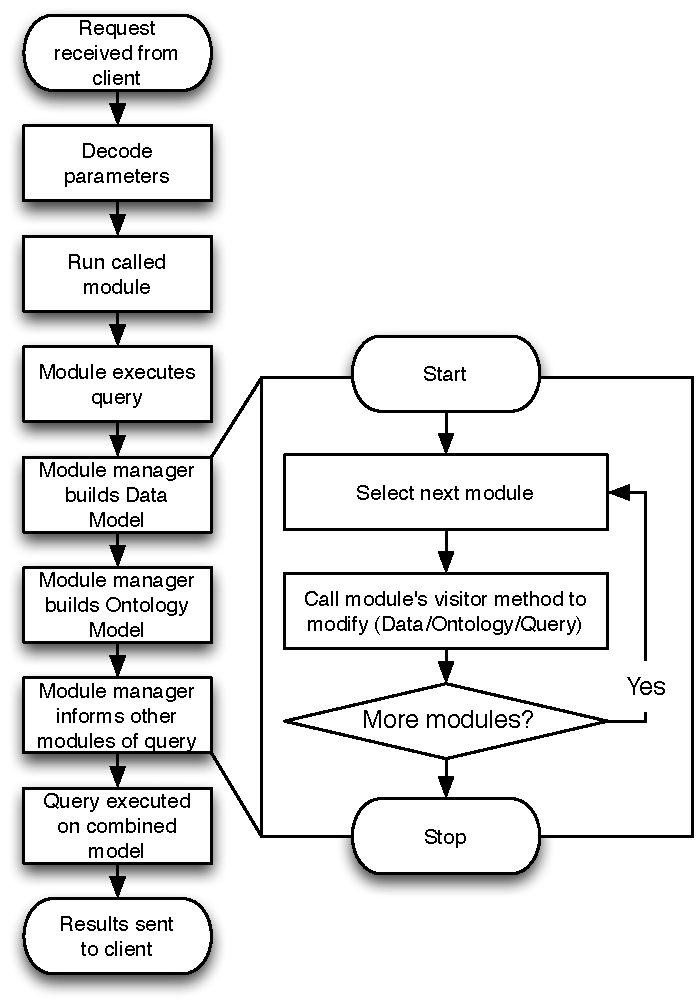
\includegraphics[width=57mm, height=78mm]{ExecutionFlow.pdf}
\caption{General overview of server-side request processing. The ModuleManager allows every module an opportunity to modify the semantic model, queries, or data model before returning results of the user's query back to the client.}
\label{execution-flow}
\end{center}\end{figure}

\section{The ProvidesDomain Interface}
\index{ProvidesDomain@\texttt{ProvidesDomain}|textbf}
\index{module!SemantEco!data provider}
Domains are an integral part of the SemantEco architecture and provide a mechanism for users of SemantEco to appropriately narrow down queries to data relevant to their needs. If a module is going to provide data for a domain, it must implement the \texttt{ProvidesDomain} interface. This interface requires a single method, \texttt{getDomains}, that the module must implement to return the domains it provides. Listing~\ref{listing:ProvidesDomain} provides sample code of how this is accomplished in the water data provider module and may be used by developers as an exemplar of how to generate additional domains.

\begin{lstlisting}[float,style=Java,caption=Code exemplar for ProvidesDomain,label=listing:ProvidesDomain]
public static final String WATER_NS = "http://escience.rpi.edu/ontology/semanteco/2/0/water.owl#";
public static final String URI_VAR = "uri";
public static final String LABEL_VAR = "label";

public List<Domain> getDomains() {
  List<Domain> domains = new ArrayList<Domain>();
  Domain water = config.getDomain(URI.create(WATER_NS), true);
  water.setLabel("Water");
  addDataSources(water, request);
  addRegulations(water);
  addDataTypes(water);
  domains.add(water);
  return domains;
}

protected void addDataSources(Domain domain, Request request) {
  // get data sources from a remote metadata repository
  String response = queryForDataSources(request); // not shown
  try {
    JSONObject data = new JSONObject(response);
    JSONArray entries = data.getJSONArray("data");
    for(int i=0; i<entries.length(); i++) {
      JSONObject entry = entries.getJSONObject(i);
      String uri = entry.getString(URI_VAR);
      String label = entry.getString(LABEL_VAR);
      domain.addSource(URI.create(uri), label);
    }
  } catch(JSONException e) {
    log.warn("Invalid result returned from server.", e);
  }
}

protected void addRegulations(Domain domain) {
  domain.addRegulation(URI.create("http://escience.rpi.edu/ontology/semanteco/2/0/EPA-regulation.owl"),
                       "EPA Regulation");
  // repeat for additional regulations
}

protected void addDataTypes(Domain domain) {
  Resource icon = config.getResource("clean-water.png");
  domain.addDataType("clean-water", "Clean Water", icon);
  // repeat for additional data types
}
\end{lstlisting}

There are three primary goals when generating a Domain object. First, one must provide all of the data sources that are being used to provide data in the domain. In the exemplar, this is accomplished by querying a metadata graph (code not shown) and iterating over the query results and adding each into the set of data sources. An example would be the EPA, which is identified in the metadata graph as \texttt{http://sparql.tw.rpi.edu/source/epa-gov}. Second, one must define entity types. These often map to classes in the underlying ontology (see Sec.~\ref{ontology-construction} for more details on defining an ontology), such as \textit{WaterSite} or \textit{PollutedFacility} in the case of the water data provider. Entity types are composed of a unique identifier that must conform to HTML requirements for identifiers,\footnote{We recommend using only alphanumeric characters and the hyphen (-) character} a label presented to the user, and a resource object used to represent entities of the entity type in the facet interfaces or on the map. Lastly, one must generate 

\section{Ontology Construction}
\label{ontology-construction}
In this section we provide examples of classes that extend the SemantEco ontology as a basis for discussing how module designers can similarly extend the ontology to model new domains.
\section{Data Conversion}
In this section we provide instructions for converting data using CSV2RDF4LOD \cite{lebo2011producing} and include some sample enhancements from previous conversions.
\section{Visitor Methods}
\label{visitors}
In this section we present a detailed discussion of the different visitor methods that modules must provide.
\subsection{Adding client interfaces and behavior}
In this subsection we outline how to add scripts, stylesheets, and facets to the SemantEco user interface via the UI visitor.
\subsection{Populating the Data Model}
In this subsection we demonstrate how to read data from an external triple store into the local model so that it will be exposed to the other modules and available for any local queries.
\subsection{Extending the Ontology Model}
In this subsection we demonstrate how to extend the ontology model by reading in external ontologies using Jena \cite{Jena}.
\subsection{Augmenting Queries from other Modules}
In this subsection we discuss how to augment queries and use the metaquery methods exposed by the \texttt{Query} object to make decisions about what modifications, if any, should be performed.
\section{Exceptional Behavior}
In this section we discuss alternative behaviors for loading and querying data and the reasons why one might want to use them over the visitor methods outlined in the previous section.




\chapter{Available Modules}
In this chapter we will provide an in-depth look at the current set of modules for SemantEco and the different datasets and query methods they provide. We will also discuss the different classifications of modules (i.e. core, data provider, and query-altering).
\section{Core Modules}
This section will discuss the core modules that are required in the general flow of SemantEco. Removing any of these modules will break the user interface as it is currently engineered (although in many cases an alternative module could be supplied).
\subsection{Domain Module}
In this subsection we discuss the domain module's purpose.
\subsection{Data Source Module}
In this subsection we discuss the data source module's purpose.
\subsection{Regulation Module}
In this subsection we discuss the regulation module's purpose and query methods.
\subsection{Entity Type Module}
In this subsection we discuss the entity type module's purpose.
\subsection{Zip Code Module}
In this subsection we discuss the zip code module's purpose and query methods.
\subsection{Debugger Module}
In this subsection we discuss the debugger module and how module designers can use it to assist in debugging modules.
\section{Data Provider Modules}
In this section we discuss data provider modules and how they provide data and ontologies to SemantEco through the various visitor methods discussed in Section~\ref{visitors}.
\subsection{Water Data Provider}
In this subsection we discuss the water data provider, its ontologies, and its data sources.
\subsection{Air Data Provider}
In this subsection we discuss the air data provider, its ontologies, and its data sources.
\subsection{Species Data Provider}
In this subsection we discuss the species data provider, its ontologies, and its data sources. We also discuss its use of the hierarchical search facet to assist users in locating data.
\section{Query-modifying Modules}
In this section we discuss modules that do not provide additional data, but instead make use of the query visitor pattern to augment queries from other modules to restrict them to certain criteria.
\subsection{Time Module}
In this subsection we discuss the time module and how it modifies queries pertaining to measurements to limit them to certain time frames.
\subsection{Industry Module}
In this subsection we discuss the industry module and how it uses North American Industry Classification System (NAICS) to restrict queries regarding facilities to those facilities in a particular industry.
\subsection{Characteristic Module}
In this subsection we discuss the characteristic module and its ontology that merges ChEBI and SNOMED. Furthermore, we discuss the use of this ontology in a hierarchical search facet.
\chapter{Conclusions}
In this chapter we will present our conclusions.

\appendix
\chapter{Maven Build System}
\label{maven-build-system}\index{Maven|textbf}
SemantEco uses the Apache Maven\footnote{\url{http://maven.apache.org/}} build system to handle its build process. SemantEco is composed of a number of Maven modules, and the published artifacts are available via an Artifactory repository hosted by the Tetherless World.\footnote{\url{https://orion.tw.rpi.edu/artifactory/}} Instructions for downloading and installing Maven can be found on the Maven website\footnote{\url{http://maven.apache.org/download.cgi}} and there are additional configuration information for the SemantEco project hosted on the Tetherless World's website.\footnote{\url{http://tw.rpi.edu/web/project/SemantEco/maven}}

\section{Standalone Modules}
Each component of SemantEco is a module in a top-level Maven POM file. Development of stand-alone modules can reference the build artifacts via Tetherless World's Artifactory installation. To do so, one must put the following snippet in their module's pom.xml:

\begin{lstlisting}
<repositories>
  <repository>
    <id>tetherless</id>
    <url>http://orion.tw.rpi.edu/artifactory/libs-release</url>
    <releases><enabled>true</enabled></releases>
    <snapshots><enabled>false</enabled></snapshots>
  </repository>
  <repository>
    <id>tetherless-snapshots</id>
    <url>http://orion.tw.rpi.edu/artifactory/libs-snapshot</url>
    <releases><enabled>false</enabled></releases>
    <snapshots><enabled>true</enabled></snapshots>
  </repository>
</repositories>
\end{lstlisting}

\noindent Note: This step is not required if you have added your module to the existing SemantEco repository as this step has already been done in the root pom.xml.

\section{Build-time Profiles and Application Configuration}
SemantEco has two Maven profiles that control its build process. The default profile is for development purposes and is configured to deploy the SemantEco WAR file to a local servlet container instance. The development profile also includes the \texttt{Debugger} module that provides an alternate interface for testing SPARQL queries against Pellet-backed data models. The second profile is for production deployment. It is configured specifically for SemantEco deployment at the Tetherless World Constellation, so its parameters should be adjusted according to the environment where it is set to be deployed. To build a production version, one must tell Maven to activate it via the \texttt{-P} command line parameter (i.e. \texttt{mvn clean install -P production}).

Additionally, SemantEco has a number of properties that govern its behavior at run time. It reads these properties from a file called semanteco.properties. These properties come from the \texttt{<properties>} element in the webapp's pom.xml file. As of this writing, the current set of properties are:

\begin{itemize}
\item \textbf{debug} This is set by development mode and increases the amount of logging performed by the application for debugging purposes.
\item \textbf{triple-store} The default triple store to execute queries against. In development it points to \url{http://was.tw.rpi.edu/virtuoso/sparql} and in production points to \url{http://localhost:3003/}.
\item \textbf{baseUrl} The base URL is the user-facing path for SemantEco. It uses this to construct its RESTful URLs for client-server communication. This should not be present in development. The default for production is \url{http://aquarius.tw.rpi.edu/projects/semanteco/}.
\end{itemize}

In addition to these properties, SemantEco also consumes a single environment variable, \texttt{semantEcoRootPath}, that defaults to its location within the servlet container's webapps directory. This is used for SemantEco to generate logs, and changing it will change where the log files are stored.

\chapter{Source Code Management}
The original line of SemantEco software was developed and maintained at Google Code.\footnote{\url{http://code.google.com/p/swqp/}} Due to the success of the project and the large number of exploratory offshoots, it was necessary to move to a faster source code management system. To this end, SemantEco has been migrated to use the Git source code management tool to maintain its source history. The project is hosted via Github at \url{https://github.com/ewpatton/SemantEco} and maintains the entire history of the project, including the original Subversion repository from Google Code.

Parties interested in submitting code to SemantEco should use the Github application to fork the repository and submit pull requests back to the main repository. The main repository uses the Git Flow\footnote{\url{http://nvie.com/posts/a-successful-git-branching-model/}} development paradigm, so pull requests should point to a branch from \texttt{develop} that contains the necessary code for the feature. Multiple features should be submitted on multiple branches. Experts may feel free to use command-line Git but are discouraged from rebasing unless absolutely necessary. Any pull requests that would cause conflicts with \texttt{develop} or fail unit tests will be rejected.

\cleardoublepage
\addcontentsline{toc}{chapter}{References}
\renewcommand{\bibname}{References}
\bibliographystyle{ieeetr}
\bibliography{Semanteco}

\index{QueryExecutor@\texttt{QueryExecutor}|seealso{query, executing}}
\cleardoublepage
\addcontentsline{toc}{chapter}{Index}
\printindex
\end{document}